\documentclass[11pt,a4paper]{article}
\usepackage[utf8]{inputenc}
\usepackage[margin=1in]{geometry}
\usepackage{amsmath}
\usepackage{amssymb}
\usepackage{booktabs}
\usepackage{hyperref}
\usepackage{microtype}
\usepackage{titlesec}
\usepackage{tcolorbox}
\usepackage{listings}
\usepackage{color}

% Custom Colors
\definecolor{primary}{RGB}{15, 23, 42}      % Slate 900
\definecolor{secondary}{RGB}{71, 85, 105}   % Slate 600
\definecolor{accent}{RGB}{14, 116, 144}     % Cyan 700
\definecolor{bglight}{RGB}{248, 250, 252}   % Slate 50

\hypersetup{
    colorlinks=true,
    linkcolor=accent,
    filecolor=accent,
    urlcolor=accent,
    citecolor=accent
}

% Title Formatting
\titleformat{\section}{\large\bfseries\color{primary}}{\thesection}{1em}{}
\titleformat{\subsection}{\normalsize\bfseries\color{accent}}{\thesubsection}{1em}{}
\titleformat{\subsubsection}{\small\bfseries\color{secondary}}{\thesubsubsection}{1em}{}

% Listings Styling
\lstset{
    backgroundcolor=\color{bglight},
    basicstyle=\small\ttfamily,
    breaklines=true,
    captionpos=b,
    commentstyle=\color{secondary},
    keywordstyle=\color{accent},
    stringstyle=\color{highlight},
    frame=single,
    rulecolor=\color{secondary!30}
}

\title{
    \vspace{-2cm}
    \textbf{Comprehensive Presenter's Study Guide: Query-Independent Sentence Salience}\\
    \large Core Theories, Mathematical Formulations, Architecture Details, and Academic Q\&A
}
\author{\textbf{Madduru Nikhil} \\ Sentence Salience Research Project}
\date{\today}

\begin{document}

\maketitle

\begin{tcolorbox}[colback=bglight,colframe=accent,title=Purpose of this Document]
This comprehensive guide is created to prepare you for your research presentation. It contains detailed theoretical chapters, step-by-step algorithms, mathematical proofs and formulations, and a mock defense Q\&A section containing over 30 difficult questions that professors are likely to ask during your defense.
\end{tcolorbox}

\tableofcontents
\newpage

\section{Introduction and Project Scope}

\subsection{The Downstream Application: Query-Independent Question Generation}
In standard Question Answering (QA) and Question Generation (QG) pipelines, models rely on user queries or keyword overlaps to locate relevant information. However, in **Query-Independent Question Generation**, the task is to identify answer-worthy, high-information sentences from a source document \textit{before} any question is formulated.

This is a critical preprocessing step for automated tutoring, automated exam generation, and document summarization. If the salience selector fails (i.e., misses a key fact), the downstream QG model can never generate a question about that fact. Therefore, our target is to maximize **Recall** (capturing all facts) while maintaining high ranking quality (**MAP** and **NDCG**).

\subsection{Why Exclude Alignment Features?}
Standard text models use query-document alignment features (such as cosine similarity of TF-IDF vectors or word overlaps) to flag important sentences. 
In our research, we **explicitly exclude all alignment features** (`align\_` variables). 
* **The Reason**: We want the model to learn the intrinsic structural properties of a sentence that make it salient, regardless of user queries.
* **The Challenge**: Without alignment shortcuts, the model must rely purely on discourse structure, syntax, semantics, and information-theoretic density.

---

\section{Rhetorical Structure Theory (RST) in Depth}

Rhetorical Structure Theory (RST), originally proposed by Mann and Thompson (1988), is a hierarchical model of text organization. It describes the discourse relations that hold between text spans.

\subsection{Structural Units}
* **Elementary Discourse Units (EDUs)**: The leaf nodes of the discourse tree. An EDU is typically a clause containing a single verb phrase.
* **Span**: A text block consisting of one or more adjacent EDUs.
* **Nucleus (N)**: The essential part of a relation. If a Satellite is deleted, the text remains comprehensible. If a Nucleus is deleted, the text becomes incoherent.
* **Satellite (S)**: The auxiliary, supporting text span.

\subsection{Common Discourse Relations}
Our model extracts features based on specific rhetorical relations identified by the parser:
\begin{itemize}
    \item \textbf{Elaboration}: The Satellite provides additional details about the Nucleus. This is the most common relation in narrative text.
    \item \textbf{Attribution}: The Satellite credits a source for the statement in the Nucleus (e.g., \textit{"Researchers announced that [N]..."}).
    \item \textbf{Background}: The Satellite provides historical or contextual information necessary to understand the Nucleus.
    \item \textbf{Contrast}: A multinuclear relation where two spans are compared to show differences.
    \item \textbf{Joint}: A multinuclear relation linking independent items in a list.
\end{itemize}

\subsection{Discourse Features Extracted}
We extract structural statistics from the RST tree for each sentence:
\begin{enumerate}
    \item \textbf{RST Depth}: The height of the sentence node in the parse tree. Sentences close to the root (depth $\le 2$) represent main discourse topics.
    \item \textbf{Nucleus count (`rst\_n\_count`) \& Satellite count (`rst\_s\_count`)}: The number of Nucleus and Satellite nodes within the sentence boundaries.
    \item \textbf{Nucleus-to-Leaf Ratio}: A high ratio indicates that the sentence consists mostly of core information rather than subordinate clauses.
\end{enumerate}

---

\section{Information Theory and Cognitive Surprisal}

Information theory provides a mathematical framework for measuring the information content of language.

\subsection{Mathematical Formulation of Surprisal}
According to Shannon’s information theory, the information content (or surprisal) of a word $w_t$ in a context of preceding words $w_{<t}$ is defined as:
\[
I(w_t) = -\log_2 P(w_t \mid w_{<t})
\]
If a word is highly predictable ($P \approx 1$), its surprisal is close to 0. If a word is highly unexpected ($P \approx 0$), its surprisal is large.

\subsection{Causal vs. Masked Surprisal}
We use two different language models to extract surprisal features:
\begin{enumerate}
    \item \textbf{Causal Surprisal (GPT-2)}: Generates surprisal left-to-right. It models how a human reader processes text sequentially.
    \item \textbf{Masked Pseudo-Log-Likelihood (PLL) (BERT)}: Measures the bi-directional predictability of a token. We mask token $w_t$ and calculate its probability given both preceding and following context:
    \[
    \text{PLL}(w_t) = -\log_2 P(w_t \mid w_{\setminus t})
    \]
\end{enumerate}

\subsection{Uniform Information Density (UID)}
The UID hypothesis (Jaeger, 2010) states that speakers structure their sentences to maintain a relatively constant rate of information transmission close to the channel capacity. 
* **Application**: Salient sentences carry a high density of information (reflected in higher tail surprisals at the 90th and 95th percentiles).
* **Surprisal Difference**: Smooth surprisal transitions (low variance/difference between consecutive tokens) correlate with high salience because they represent efficient, uniform information distribution.

\subsection{Sentence Deletion Coherence Drop}
This feature measures the degradation of context cohesion when the target sentence is removed. Let $P$ be the context passage and $S_i$ be the $i$-th sentence:
\[
\text{Drop}(S_i) = \text{MeanSurprisal}(P \setminus \{S_i\}) - \text{MeanSurprisal}(P)
\]
A large positive drop indicates that the surrounding sentences became much harder for the language model to predict, proving that $S_i$ was a crucial semantic bridge.

---

\section{Dataset Biases and Feature Engineering}

\subsection{Lead Position Bias}
SQuAD passages suffer from strong positional bias:
\begin{table}[h]
    \centering
    \begin{tabular}{cc}
        \toprule
        \textbf{Sentence Index} & \textbf{Percentage of Salient Sentences (\%)} \\
        \midrule
        0 & 28.5\% \\
        1 & 21.3\% \\
        2 & 16.5\% \\
        3 & 12.1\% \\
        4+ & 21.6\% \\
        \bottomrule
    \end{tabular}
\end{table}
If trained on raw unbalanced data, machine learning models will simply learn to predict "salient" for the first two sentences and "non-salient" for the rest, ignoring content.

\subsection{Feature Families}
We extract 71 non-alignment features grouped into five families:
\begin{enumerate}
    \item \textbf{Discourse (RST)}: Tree depth, nucleus/satellite counts, relation tags.
    \item \textbf{Cognitive Surprisal}: Sum, mean, max, standard deviation, and tail percentiles of GPT-2 and BERT surprisals.
    \item \textbf{Concreteness}: Lemmatized words matched against the Brysbaert 40,000 word lexicon. Salient sentences contain concrete nouns (e.g., "oxygen", "oxygenation") rather than abstract concepts.
    \item \textbf{Sentiment Polarity}: VADER polarity scores (positive, negative, neutral, and compound).
    \item \textbf{Linguistic \& Syntactic}: Word count, character count, POS tag ratios, and parse tree depth.
\end{enumerate}

---

\section{Dataset Balancing Algorithms}

To eliminate lead position bias and handle class imbalance, we evaluate five balancing algorithms:

\subsection{Discourse-Semantic Neighborhood Balancing (DSNB)}
DSNB is our proposed balancing method. It selects highly informative, local negative samples to force the model to learn content differences.

\begin{lstlisting}[language=Python, caption=DSNB Negative Sampling Algorithm]
def apply_dsnb(contexts, salient_sentences, non_salient_sentences):
    balanced_dataset = []
    for context in contexts:
        # Step 1: Identify salient sentences in this context
        positives = [s for s in context if s.label == 1]
        negatives = [s for s in context if s.label == 0]
        
        for pos in positives:
            # Step 2: Find discourse neighbors (adjacent in RST tree)
            neighbors = get_rst_neighbors(pos, negatives)
            
            if not neighbors:
                # Fallback to physical adjacent sentences
                neighbors = get_adjacent_sentences(pos, negatives)
                
            # Step 3: Compute semantic similarity using embeddings
            similarities = []
            for neg in neighbors:
                sim = cosine_similarity(pos.embedding, neg.embedding)
                similarities.append((sim, neg))
                
            # Sort neighbors by similarity (highest first)
            similarities.sort(key=lambda x: x[0], reverse=True)
            
            # Step 4: Sample the hardest semantic negative
            hardest_negative = similarities[0][1]
            
            balanced_dataset.append(pos)
            balanced_dataset.append(hardest_negative)
            
    return balanced_dataset
\end{lstlisting}

---

\section{Model Architectures and Mathematical Formulations}

\subsection{Hybrid Gated BERT (Config 6)}
Gated BERT uses a learnable gating vector to dynamically weight semantic CLS embeddings and explicit feature representations.

\subsubsection{Gated BERT Mathematical Flow}
Let $h_{\text{bert}} \in \mathbb{R}^{768}$ be the BERT CLS embedding. Let $h_{\text{tab}} \in \mathbb{R}^{71}$ be the explicit feature vector.
1. Project the explicit features to the same dimensions as BERT:
\[
h_{\text{tab\_proj}} = \text{LeakyReLU}(W_p h_{\text{tab}} + b_p) \quad \text{where } W_p \in \mathbb{R}^{768 \times 71}
\]
2. Compute the gating vector $g \in (0, 1)^{768}$:
\[
g = \sigma(W_g [h_{\text{bert}}; h_{\text{tab\_proj}}] + b_g) \quad \text{where } W_g \in \mathbb{R}^{768 \times 1536}
\]
3. Fuse the vectors element-wise:
\[
h_{\text{fused}} = g \odot h_{\text{bert}} + (1 - g) \odot h_{\text{tab\_proj}}
\]
4. Pass through the final classification layer:
\[
p = \sigma(W_c h_{\text{fused}} + b_c) \quad \text{where } W_c \in \mathbb{R}^{1 \times 768}
\]

---

\subsection{FiLM BERT (Config 7)}
Feature-wise Linear Modulation (FiLM) modulates BERT activation using explicit features.

\subsubsection{FiLM Mathematical Flow}
1. Generate scale ($\gamma$) and shift ($\beta$) vectors from explicit features:
\[
\gamma = W_\gamma h_{\text{tab}} + b_\gamma, \quad \beta = W_\beta h_{\text{tab}} + b_\beta \quad \text{where } \gamma, \beta \in \mathbb{R}^{768}
\]
2. Modulate the BERT embedding:
\[
h_{\text{mod}} = \gamma \odot h_{\text{bert}} + \beta
\]
3. Concatenate with a skip connection:
\[
h_{\text{fused}} = [h_{\text{mod}}; h_{\text{tab}}]
\]
4. Classification:
\[
p = \sigma(W_c h_{\text{fused}} + b_c)
\]

---

\subsection{LGSM (Language-Guided Salience Model - Config 12)}
LGSM is a sequence-to-sequence selector designed to capture passage-level dependencies.

\subsubsection{LGSM Mathematical Flow}
For a passage with $N$ sentences:
1. Dynamic Gate:
\[
\alpha_t = \sigma(W_a [h_{\text{bert}, t}; \text{MLP}(h_{\text{tab}, t})] + b_a) \quad \text{where } \alpha_t \in \mathbb{R}^1
\]
\[
x_t = \alpha_t \cdot h_{\text{bert}, t} + (1 - \alpha_t) \cdot \text{MLP}(h_{\text{tab}, t}) \quad \text{where } x_t \in \mathbb{R}^{768}
\]
2. Add Sinusoidal Positional Encoding:
\[
PE_{(pos, 2i)} = \sin\left(\frac{pos}{10000^{2i/768}}\right), \quad PE_{(pos, 2i+1)} = \cos\left(\frac{pos}{10000^{2i/768}}\right)
\]
\[
z_t = x_t + PE_t
\]
3. Sequence Transformer:
Pass sequence $Z = [z_1, \dots, z_N]$ through a 2-layer Transformer Encoder:
\[
H = \text{TransformerEncoder}(Z) \quad \text{where } H \in \mathbb{R}^{N \times 768}
\]
4. Classification with Focal Loss:
To handle remaining class imbalances, we train using Binary Focal Loss:
\[
\mathcal{L} = -\sum_{t=1}^N \alpha_{\text{focal}} (1 - p_t)^\gamma y_t \log(p_t) + (1 - \alpha_{\text{focal}}) p_t^\gamma (1 - y_t) \log(1 - p_t)
\]
where $\gamma = 3.0$ and $\alpha_{\text{focal}} = 0.25$.

---

\section{The 12 Evaluated Configurations}

To provide a clear reference, here is the complete grid of the 12 model configurations evaluated in this project:

\begin{table}[h!]
    \centering
    \small
    \caption{Complete grid of the 12 evaluated model configurations with architecture design choices and best validation results. ``Best Bal.'' = balancing strategy that achieved the highest validation F1 for that config. F1 and NDCG are validation-set scores.}
    \label{tab:model_configs}
    \begin{tabular}{c l l l l c c}
        \toprule
        \textbf{ID} & \textbf{Model Type} & \textbf{Architecture} & \textbf{RST Use} & \textbf{Best Bal.} & \textbf{Val F1} & \textbf{Val NDCG} \\
        \midrule
        1  & Rule-Based      & Threshold heuristic             & Prior (hard)   & None          & 0.304 & 0.600 \\
        2  & LR (RST)        & Logistic regression             & Features       & DSNB          & 0.336 & 0.662 \\
        3  & LR (Linguistic) & Logistic regression             & Features       & Cluster       & 0.353 & 0.684 \\
        4  & LR (Surprisal)  & Logistic regression             & None           & None          & 0.325 & 0.667 \\
        5  & LR (Combined)   & Logistic regression             & Features       & RST-Nbhd      & 0.341 & 0.660 \\
        6  & Gated BERT      & Gating: $\mathbf{g}=\sigma(W_g[\mathbf{h};\mathbf{f}])$ & Concat gate & RST-Nbhd & 0.346 & 0.669 \\
        7  & FiLM BERT       & FiLM: $\gamma \odot \mathbf{h} + \beta$     & Modulation & Cluster  & 0.333 & 0.594 \\
        8  & Concat BERT     & $[\mathbf{h}_{CLS};\mathbf{f}]$ linear head & Concat feat & Pairwise & 0.329 & 0.677 \\
        9  & Gated BERT (no RST) & Gating (ablation)           & None           & Pairwise      & 0.312 & 0.635 \\
        10 & BERT Only       & BERT CLS $\rightarrow$ linear   & None           & None          & --    & --    \\
        11 & Guided BERT     & Logit fusion: $l_{final}=l_{BERT}+w \cdot h_{RST}$ & Prior (soft) & Pairwise & 0.324 & 0.666 \\
        12 & LGSM            & Sequence-level BERT transformer & Concat feat    & None          & 0.299 & 0.632 \\
        \bottomrule
    \end{tabular}
\end{table}

\section{Dataset Balancing Methods: Formulations \& Mathematical Details}

In order to train robust sentence selectors that ignore spatial patterns and focus strictly on content, class balancing is applied during training. Here we formulate each of the five balancing methods:

\subsection{None (Raw Unbalanced)}
No balancing is performed. The training objective is standard empirical risk minimization over the highly skewed original SQuAD class distribution:
\[
\mathcal{L}_{\text{None}} = \sum_{i=1}^N \mathcal{L}(y_i, f(x_i))
\]
where the imbalance ratio $\rho$ is defined as:
\[
\rho = \frac{|S_{\text{non-salient}}|}{|S_{\text{salient}}|} = \frac{2,037}{493} \approx 4.13
\]
This forces the model to heavily prioritize the majority class (non-salient), leading to high precision but low recall.

\subsection{Pairwise Balancing (Relative Ranking)}
Pairwise balancing reframes the task as a binary classification of ordered pairs. For a context passage, we construct pairs of sentences $(s_i, s_j)$ such that $s_i$ is salient ($y_i = 1$) and $s_j$ is non-salient ($y_j = 0$). 
The training goal is to predict if $s_i$ is more salient than $s_j$ using their scores $f(s_i)$ and $f(s_j)$.
The pairwise cross-entropy loss is formulated as:
\[
\mathcal{L}_{\text{Pairwise}} = -\sum_{(s_i, s_j) \in P} \log \sigma \left( f(s_i) - f(s_j) \right)
\]
where $\sigma(z) = 1 / (1 + e^{-z})$ is the sigmoid function. 
\begin{itemize}
    \item \textbf{Significance}: By training on the difference in scores, the model ignores absolute coordinates (like linear position) and learns to rank sentences relative to each other.
\end{itemize}

\subsection{Cluster-Based Balancing}
Cluster-based balancing groups the negative (non-salient) sentences into representative semantic groups, sampling one negative from each group to build a 1:1 balance.
1. We apply K-Means clustering to the explicit feature vectors of all negative sentences in the context passage:
\[
\arg\min_{\mathbf{C}} \sum_{k=1}^K \sum_{x_j \in C_k} ||x_j - \mu_k||^2
\]
where $K = |S_{\text{salient}}|$ (the number of positive sentences in that context) and $\mu_k$ is the centroid of cluster $C_k$.
2. For each cluster $C_k$, we select the sentence $s_j^*$ closest to the centroid:
\[
s_j^* = \arg\min_{s_j \in C_k} ||x_j - \mu_k||^2
\]
\begin{itemize}
    \item \textbf{Significance}: This creates a balanced training set while ensuring that the negative samples represent the full diversity (clusters) of background information in the document, avoiding redundant negatives.
\end{itemize}

\subsection{RST-Neighborhood Balancing}
This method samples negative sentences that are structurally closest to the salient sentence in the Rhetorical Structure Theory (RST) tree.
For a salient sentence $s_i$, we define the RST distance $d_{\text{RST}}(s_i, s_j)$ as the shortest path length (number of edges) between their respective nodes in the discourse tree.
We select the negative sentence $s_j^*$ that minimizes this distance:
\[
s_j^* = \arg\min_{s_j \in S_{\text{non-salient}}} d_{\text{RST}}(s_i, s_j)
\]
\begin{itemize}
    \item \textbf{Significance}: This forces the model to contrast the salient sentence with sentences that are rhetorically linked to it, making it harder for the model to use general topic differences as a shortcut.
\end{itemize}

\subsection{DSNB (Discourse-Semantic Neighborhood Balancing)}
Our proposed method, DSNB, combines structural discourse adjacency with semantic vector similarity to select the hardest, most informative local negatives:
1. Define the RST-neighborhood of a salient sentence $s_i$ as:
\[
\mathcal{N}_{\text{RST}}(s_i) = \{s_j \in S_{\text{non-salient}} \mid d_{\text{RST}}(s_i, s_j) \le \theta_{\text{RST}}\}
\]
where $\theta_{\text{RST}}$ is a tree-distance threshold (typically 2). If $\mathcal{N}_{\text{RST}}(s_i)$ is empty, we fall back to physical adjacency in the text:
\[
\mathcal{N}_{\text{physical}}(s_i) = \{s_{i-1}, s_{i+1}\}
\]
2. From this local neighborhood, we select the negative sentence $s_j^*$ that has the highest semantic similarity to $s_i$ using their vector embeddings $\mathbf{v}(s)$:
\[
s_j^* = \arg\max_{s_j \in \mathcal{N}(s_i)} \cos\left( \mathbf{v}(s_i), \mathbf{v}(s_j) \right) = \arg\max_{s_j \in \mathcal{N}(s_i)} \frac{\mathbf{v}(s_i) \cdot \mathbf{v}(s_j)}{||\mathbf{v}(s_i)|| \cdot ||\mathbf{v}(s_j)||}
\]
\begin{itemize}
    \item \textbf{Significance}: DSNB generates extremely challenging local negatives. By comparing a salient sentence with a sentence that is rhetorically adjacent and semantically similar, the model is forced to ignore general paragraph topics and focus on the fine-grained factual differences that make a sentence answer-worthy.
\end{itemize}

---

\section{Evaluation \& Ranking Metrics: Formulations \& Project Significance}

Salience selection is evaluated using both flat classification metrics (at a fixed probability threshold $\tau = 0.35$) and context-level ranking metrics.

\subsection{Flat Classification Metrics}

\subsubsection{Precision}
\[
\text{Precision} = \frac{TP}{TP + FP}
\]
\begin{itemize}
    \item \textbf{Project Significance}: Precision measures the purity of the selected sentences. Low precision means the model flags many background sentences as salient. In a downstream QG pipeline, this translates to high computational waste: the QG model will waste CPU/GPU cycles trying to generate questions from sentences that do not contain actual facts or answers.
\end{itemize}

\subsubsection{Recall}
\[
\text{Recall} = \frac{TP}{TP + FN}
\]
\begin{itemize}
    \item \textbf{Project Significance}: Recall measures the safety net of our selector. In question generation, \textbf{Recall is the most critical metric}. If a salient sentence is missed (False Negative), the downstream system can never generate a question about that fact. A high recall (like DSNB's `0.83`–`1.0`) guarantees that we capture almost all answerable information.
\end{itemize}

\subsubsection{F1-Score}
\[
\text{F1} = 2 \cdot \frac{\text{Precision} \cdot \text{Recall}}{\text{Precision} + \text{Recall}}
\]
\begin{itemize}
    \item \textbf{Project Significance}: F1 evaluates the overall classification balance. However, because we prioritize Recall over Precision, F1 alone does not tell the whole story, which is why we also evaluate ranking metrics.
\end{itemize}

\subsection{Context-Level Ranking Metrics}

Since we rank sentences within each context passage to select the top-$K$ candidates, we evaluate using ranking metrics:

\subsubsection{Mean Average Precision (MAP)}
For a context passage, let $R$ be the number of true salient sentences, and let $P(k)$ be the precision of the top-$k$ ranked list. Let $I(k)$ be an indicator function equal to 1 if the $k$-th ranked sentence is salient, and 0 otherwise:
\[
\text{AP} = \frac{1}{R} \sum_{k=1}^N P(k) \cdot I(k)
\]
\[
\text{MAP} = \frac{1}{M} \sum_{m=1}^M \text{AP}_m
\]
\begin{itemize}
    \item \textbf{Project Significance}: MAP is highly sensitive to the exact order of predictions. It heavily penalizes models that place true salient sentences at the bottom of the ranked list. A high MAP (such as Gated BERT's `0.6415`) indicates that the model puts the most question-worthy sentences at the very top.
\end{itemize}

\subsubsection{Mean Reciprocal Rank (MRR)}
For a set of $M$ context passages, let $\text{rank}_m$ be the position of the \textit{first} true salient sentence in the ranked list for passage $m$:
\[
\text{MRR} = \frac{1}{M} \sum_{m=1}^M \frac{1}{\text{rank}_m}
\]
\begin{itemize}
    \item \textbf{Project Significance}: MRR measures how quickly the model finds a single salient sentence. This is highly significant if the QG pipeline's objective is to generate \textbf{only one high-quality question per paragraph} (e.g., for quick quizzes), making the quality of the top-ranked sentence paramount.
\end{itemize}

\subsubsection{Normalized Discounted Cumulative Gain (NDCG)}
Discounted Cumulative Gain (DCG) at a rank position $p$ is defined as:
\[
\text{DCG}_p = \sum_{i=1}^p \frac{rel_i}{\log_2(i + 1)}
\]
where $rel_i \in \{0, 1\}$ is the salience label of the sentence at rank $i$. The Normalized DCG (NDCG) is:
\[
\text{NDCG}_p = \frac{\text{DCG}_p}{\text{IDCG}_p}
\]
where $\text{IDCG}_p$ is the Ideal DCG (the score achieved by a perfect ranking).
\begin{itemize}
    \item \textbf{Project Significance}: NDCG discounts correct predictions logarithmically as they appear lower in the list. This is the gold standard for evaluating multi-sentence selection when we want to generate multiple questions per passage, ensuring the highest-quality sentences appear first.
\end{itemize}

---

\section{Statistical Analyses \& Refitting Formulations}

We conduct statistical studies to mathematically justify the features and validate the annotations:

\subsection{Post-LASSO Feature Selection}
Standard LASSO applies an L1 penalty to select features:
\[
\min_{\beta} \left( \sum_{k=1}^N \mathcal{L}(y_k, \beta^T x_k) + \lambda \sum_{j=1}^D |\beta_j| \right)
\]
\begin{itemize}
    \item \textbf{The Bias}: The L1 penalty $\lambda \sum |\beta_j|$ introduces a shrinkage bias, pushing all coefficient values closer to zero. This biases the estimates and makes standard hypothesis testing (p-value calculation) invalid.
    \item \textbf{The Post-LASSO Solution}:
      1. We identify the set of active features selected by LASSO: $S = \{j \mid \beta_j \neq 0\}$.
      2. We refit an unregularized Logistic Regression model using \textit{only} the features in $S$ while forcing controls for length and position:
      \[
      \max_{\beta_S} \sum_{k=1}^N \mathcal{L}(y_k, \beta_S^T x_{k, S})
      \]
      This provides unbiased coefficient estimates ($\beta_S$) and valid standard errors, allowing us to perform the Wald test.
\end{itemize}

\subsection{Wald Hypothesis Testing}
The Wald $z$-statistic tests the null hypothesis that a feature's coefficient is zero ($H_0: \beta_j = 0$):
\[
z = \frac{\hat{\beta}_j - 0}{\text{SE}(\hat{\beta}_j)}
\]
where $\text{SE}(\hat{\beta}_j)$ is the standard error computed from the inverse Fisher Information matrix.
\begin{itemize}
    \item \textbf{Significance}: A feature is statistically significant if $|z| > 1.96$ (corresponding to $p < 0.05$). For example, information density (`rel\_surp\_causal\_pf\_sum\_ratio`) achieves $z = +4.63$ ($p < 0.00001$), mathematically proving it is not noise.
\end{itemize}

\subsection{Cohen's Kappa ($\kappa$)}
Evaluates the agreement rate between our heuristic rule-based labels and the local Qwen-1.5B LLM judge:
\[
\kappa = \frac{p_o - p_e}{1 - p_e}
\]
where $p_o$ is the observed agreement rate:
\[
p_o = \frac{\text{Number of Agreeing Samples}}{N}
\]
and $p_e$ is the expected agreement by chance:
\[
p_e = P_{\text{heuristic}}(\text{Salient}) \cdot P_{\text{LLM}}(\text{Salient}) + P_{\text{heuristic}}(\text{Non-Salient}) \cdot P_{\text{LLM}}(\text{Non-Salient})
\]
\begin{itemize}
    \item \textbf{Significance}: It controls for random agreement (e.g., if both annotators just say "non-salient" most of the time). Our Kappa of `0.44` represents moderate agreement, validating that our heuristic rules capture a coherent, non-random signal.
\end{itemize}

---

\section{Presenter's Academic Q\&A Bank (Mock Defense)}

This section contains 32 difficult questions a professor or examiner might ask you during your presentation, along with their scientific answers.

\subsection{Theory \& Motivation}

\subsubsection{Q1: Why is query-independent salience prediction a harder task than query-focused QA?}
**Answer**: In query-focused QA, the query acts as a semantic filter. The model only needs to calculate the token-level overlap or vector similarity between the query and the context to locate the answer. 
In query-independent salience prediction, the query is unknown. The model must evaluate the passage in a vacuum and determine which sentences are intrinsically informative and likely to be questioned. This requires the model to understand discourse structures, information density, and syntactic complexities, rather than relying on simple keyword alignments.

\subsubsection{Q2: Why did you exclude alignment features (`align\_`) from your models? Doesn't that hurt performance?}
**Answer**: Yes, excluding alignment features reduces raw metrics, but it is a deliberate scientific decision. SQuAD is a reading comprehension dataset where questions are written using words from the answer sentence. If we include alignment features, the model learns a trivial shortcut: matching words in the question to words in the sentence. 
By removing all alignment features, we force the model to solve the *query-independent* task: predicting salience based purely on the grammatical, rhetorical, and information-theoretic properties of the sentence.

\subsubsection{Q3: Explain the Uniform Information Density (UID) hypothesis. How does it relate to your surprisal features?}
**Answer**: The UID hypothesis states that language users prefer to distribute information (surprisal) evenly across a linguistic sequence to maximize communication efficiency without overloading the channel. 
In our feature space, this is reflected in the surprisal differences between consecutive tokens (`rel\_surp\_causal\_pf\_diff`). Our models find that salient sentences have smaller surprisal differences. This means they distribute information smoothly, avoiding extreme peaks and valleys, which makes them cognitively easier to process and highly suitable for question generation.

\subsubsection{Q4: What is the difference between causal surprisal and masked surprisal (PLL) in your feature extraction?}
**Answer**: Causal surprisal (calculated using GPT-2) computes the probability of a word given only its left-hand context. It simulates a human reading a sentence sequentially. 
Masked surprisal (Pseudo-Log-Likelihood, calculated using BERT) computes the probability of a word given both its left and right context by masking the target token. PLL captures bidirectional coherence and syntactic fits, which helps the model evaluate how well a sentence integrates into the global passage context.

\subsubsection{Q5: Why does deleting a salient sentence cause a "coherence drop"? How is this calculated?}
**Answer**: A passage is coherent when its sentences flow logically and predict each other. If you delete a sentence that serves as an essential semantic bridge or introduces key facts, the remaining text becomes disjointed. 
We calculate this by measuring the average token-level surprisal of the entire passage before and after deleting the target sentence. If deleting the sentence causes the average surprisal of the remaining tokens to increase (coherence drop), it proves the sentence carried essential contextual information.

---

\subsection{Feature Engineering \& RST}

\subsubsection{Q6: Rhetorical Structure Theory (RST) was designed for human text analysis. How does a parser automate this, and what errors does it introduce?}
**Answer**: We use the `isanlp\_rst\_v3` parser, which utilizes a deep neural transformer to predict EDU segmentations, nuclearity, and rhetorical relations (e.g., Elaboration, Attribution). 
While neural parsers are fast, they do introduce errors, such as misclassifying long-distance dependencies or confusing subtle relations (e.g., confusing *Cause* with *Background*). However, by extracting aggregated statistics (like RST tree depth and nucleus-to-leaf ratios) rather than relying on single predicted relations, our models remain robust to parser noise.

\subsubsection{Q7: Why does a negative coefficient for `rel\_rst\_depth\_ratio` ($-0.4352$) indicate high salience?}
**Answer**: In an RST parse tree, the root represents the main nucleus of the text, while deeper nodes represent subordinate details (Satellites). A negative coefficient means that sentences located at shallower depths (closer to the root) are more likely to be salient. This matches our discourse theory: the primary claims of a paragraph reside near the root, while background noise is pushed to the leaves.

\subsubsection{Q8: How does the Brysbaert Concreteness Lexicon help in predicting sentence salience?}
**Answer**: The Brysbaert lexicon contains human-annotated concreteness ratings for 40,000 English words on a scale from 1 (abstract, e.g., "concept") to 5 (concrete, e.g., "apple"). 
Salient sentences in reading comprehension datasets tend to contain specific, concrete entities (names, places, dates, physical objects) because these are easy to write questions about. Background sentences often contain abstract explanations. Thus, a higher mean concreteness score is a positive predictor of salience.

\subsubsection{Q9: Why is `sentiment\_polarity\_compound` a positive predictor of salience in your LR model?}
**Answer**: SQuAD passages contain highly descriptive, factual narratives. Sentences that carry strong descriptions often contain emotional or qualitative adjectives, which skew VADER's compound sentiment score. The positive coefficient shows that the model uses this feature as a proxy for descriptive complexity.

\subsubsection{Q10: Since character count (`char\_count`) is a positive predictor, does your model simply favor long sentences?}
**Answer**: While character count has a positive coefficient (`+0.3604`), the model does not simply favor long sentences. This is because we control for length by including features like `flesch\_kincaid\_grade` and the raw surprisal sum (`surp\_causal\_pf\_sum`), which has a negative coefficient (`-0.4473`). The negative weight on the raw surprisal sum acts as a penalty for long sentences that are made up of easy, predictable words, ensuring the model selects sentences that are long *and* information-dense.

---

\subsection{Dataset Balancing \& DSNB}

\subsubsection{Q11: SQuAD has a 19.5\% positive rate. Why is training on raw unbalanced data bad for this task?}
**Answer**: Under severe class imbalance (80.5\% negative), a classifier trained on raw data minimizes loss by becoming extremely conservative. It learns to predict the majority class (non-salient) almost all the time. 
This leads to a model with very high Precision (it is only positive when it is absolutely sure) but extremely low Recall (it misses 75\% of the salient sentences). In a question generation pipeline, a low recall is unacceptable because it means most of the document's facts are ignored.

\subsubsection{Q12: How does DSNB differ from standard random under-sampling?}
**Answer**: Random under-sampling selects negative sentences randomly from across the entire dataset. This does not help the model resolve local biases (like the lead position bias) and often introduces irrelevant negatives. 
DSNB restricts negative sampling to the **immediate discourse-semantic neighborhood** of each positive sentence. By selecting negatives that are structurally close (RST neighbors) and semantically similar (high cosine similarity), DSNB forces the model to learn the subtle content differences that distinguish a salient sentence from its immediate context, neutralizing spatial shortcuts.

\subsubsection{Q13: Why does the coefficient of `surp\_deletion\_drop` flip from positive (`+0.20` in Pairwise) to negative (`-0.31` in DSNB)?}
**Answer**: This sign flip is a direct result of neutralizing positional bias:
* In Pairwise or unbalanced setups, the model uses a positive coefficient because sentences at the beginning of paragraphs introduce new topics. Deleting them disrupts global passage coherence (high deletion drop).
* In DSNB, we pair salient sentences with non-salient sentences from the *same* paragraph. Within a local paragraph, transitional sentences have high deletion drops, whereas specific fact-carrying sentences (salient targets) introduce detail-level information. By assigning a negative coefficient under DSNB, the model filters out these general transitional sentences to isolate the factual, answer-worthy sentences.

\subsubsection{Q14: Pairwise balancing also achieves 1:1 balance. Why is DSNB superior?}
**Answer**: Pairwise balancing pairs sentences but evaluates them in a relative ranking formulation. While effective, it does not build a stable binary classification boundary, and evaluated on flat classification at a fixed threshold (like `0.35`), it over-predicts positives (leading to low precision). 
DSNB, on the other hand, selects the single hardest semantic neighbor as a negative sample, building a robust binary classification boundary that maintains high ranking performance (MAP/MRR) while controlling classification metrics.

\subsubsection{Q15: How does RST-Neighborhood balancing handle contexts where the RST parse tree is disconnected?}
**Answer**: If the RST parser fails to generate a single connected tree or if a sentence is isolated, the DSNB algorithm falls back to physical adjacent sentences (sentences immediately preceding or following the salient sentence) as its neighborhood before applying semantic similarity filtering. This guarantees that we always select local negatives.

---

\subsection{Architectures}

\subsubsection{Q16: In Gated BERT, how does the gate vector $g$ prevent the tab features from being overwhelmed by the 768-dimensional BERT CLS embedding?}
**Answer**: The gating vector $g \in (0, 1)^{768}$ is calculated dynamically using a projection of the explicit features:
\[
g = \sigma(W_g [h_{\text{bert}}; h_{\text{tab\_proj}}] + b_g)
\]
Because the gate is calculated element-wise, the model can choose to block semantic dimensions of the BERT CLS embedding and replace them with explicit discourse or surprisal features. The projection layer ($W_p$) expands the 71 explicit features to 768 dimensions before gating, ensuring both modalities have equal capacity.

\subsubsection{Q17: What is the advantage of FiLM (Feature-wise Linear Modulation) over simple vector concatenation?}
**Answer**: Simple concatenation ($[h_{\text{bert}}; h_{\text{tab}}]$) forces the classification layers to learn interaction terms between semantic and explicit features from scratch. 
FiLM uses explicit features to directly scale ($\gamma$) and shift ($\beta$) the BERT activations:
\[
h_{\text{mod}} = \gamma \odot h_{\text{bert}} + \beta
\]
This allows the explicit features to perform mathematical operations (like scaling neural activations) before the classification layer, making it much easier for the network to learn complex, non-linear interactions.

\subsubsection{Q18: Guided BERT (Config 11) fuses priors at the logit level. Why is this useful compared to representation fusion?}
**Answer**: Logit-level fusion ($logit_{\text{final}} = logit_{\text{bert}} + w_h \cdot h_{\text{score}}$) is a highly efficient, interpretability-focused architecture:
* It does not modify BERT's internal representations, meaning we do not need to retrain or fine-tune the heavy transformer layers.
* It allows us to directly inspect the weight ($w_h$) assigned to the heuristic prior, providing clear scientific insight into how much the model relies on discourse rules compared to deep semantic cues.

\subsubsection{Q19: LGSM uses Binary Focal Loss instead of Cross-Entropy. What is the mathematical benefit of this?}
**Answer**: Standard Cross-Entropy treats all classification errors equally. In highly imbalanced datasets, the loss is dominated by the easy negative examples. 
Focal Loss introduces a modulating factor $(1 - p_t)^\gamma$:
\[
\mathcal{L} = -(1 - p_t)^\gamma \log(p_t)
\]
When a negative sample is easily classified ($p_t \approx 0$ for a negative, or $1-p_t \approx 0$), the modulating factor goes to 0, down-weighting its contribution to the loss. This forces the model to focus training gradients on hard, ambiguous examples (the boundary cases).

\subsubsection{Q20: Why did you use a sequence-level Transformer in LGSM instead of treating each sentence independently?}
**Answer**: Sentence salience is not independent; it is relative to the rest of the passage. A sentence is salient because it stands out compared to its neighbors. 
By using a Sequence Transformer, LGSM can look at the entire passage sequence ($S_1, \dots, S_N$). The self-attention layers allow the model to compare each sentence's semantic and explicit features to all other sentences in the context, capturing the global flow of information.

---

\subsection{Statistics \& Evaluation}

\subsubsection{Q21: Why do you report 5-fold cross-validation at the context level instead of the sentence level?}
**Answer**: If we split the dataset randomly at the sentence level, sentences from the same context passage would end up in both the training and validation sets. Since sentences in the same passage share vocabulary, topics, and discourse structures, this would cause **data leakage**, resulting in artificially inflated validation scores. 
By splitting at the context level, we ensure that the model is validated on completely unseen passages, proving its ability to generalize.

\subsubsection{Q22: Explain the difference between MAP and NDCG. Why are they better than F1 for your application?}
**Answer**: F1 is a classification metric evaluated at a single threshold (e.g., `0.35`). It does not measure the model's ability to rank sentences. 
* **MAP (Mean Average Precision)** evaluates the precision at each correct salient sentence in the ranked list. It heavily penalizes models if they rank a salient sentence low.
* **NDCG (Normalized Discounted Cumulative Gain)** measures the gain of a sentence based on its position, using a logarithmic discount. 
Because our downstream application (Question Generation) selects the top-$K$ most salient sentences to generate questions, ranking is more important than flat classification. MAP and NDCG measure exactly how well the model puts the best sentences at the very top.

\subsubsection{Q23: How does the Wald test justify your feature selection in the post-LASSO study?}
**Answer**: Standard LASSO selects features by applying an L1 penalty, but it shrinks all coefficients toward zero (introducing regularization bias), which invalidates standard p-value calculations. 
The post-LASSO method runs an unregularized Logistic Regression *only* on the selected features. We can then apply the Wald test ($z = \beta/\text{SE}$) to calculate unbiased p-values and standard errors, proving that features like information density and satellite relations are statistically significant predictors even when controlling for sentence length and position.

\subsubsection{Q24: Your Cohen's Kappa score is 0.44. Isn't that low?}
**Answer**: In subjective NLP tasks (like salience or summarization), agreement is naturally lower than in simple tasks. A Kappa of `0.44` represents **moderate agreement** between the heuristic labels and the LLM-as-a-judge (Qwen). 
Considering that SQuAD salient sentences are defined implicitly by whatever sentences humans chose to write questions about (which is highly subjective), a moderate agreement rate of 82.00\% ($\kappa = 0.44$) shows that our heuristic rules capture a statistically significant, coherent signal.

\subsubsection{Q25: What is the optimal threshold for LGSM, and how did you determine it?}
**Answer**: Our Threshold Sensitivity Sweep (Slide 14) shows that the optimal threshold for LGSM to maximize F1 is **`0.30`** (yielding an F1 of `0.2985`). At higher thresholds (e.g., `0.50`), the model's recall drops drastically due to majority-class conservatism.

---

\subsection{Future Work \& Scaling}

\subsubsection{Q26: Why do you expect precision to increase when you scale from 100 to 500 contexts?}
**Answer**: In our 100-context experiment, the models have access to only 493 positive examples, which limits their ability to learn robust negative boundaries. 
Scaling to 500 contexts increases the training set to ~13,000 sentences (with ~2,500 positives). This larger sample size reduces vocabulary memorization and helps the models learn clean boundary features, which will significantly reduce false positives and increase validation Precision.

\subsubsection{Q27: How will you evaluate the downstream QG quality in your future work?}
**Answer**: We will plug our salience selector into a pre-trained T5-base QG model. We will generate questions from the sentences selected by our model and compare them to the gold-standard SQuAD questions using automated translation metrics:
* **BLEU-4**: Measures 4-gram overlap.
* **ROUGE-L**: Measures longest common subsequence.
* **METEOR**: Measures semantic alignment and synonyms.

\subsubsection{Q28: How does your approach handle multi-paragraph documents?}
**Answer**: Currently, our model processes text at the context-passage level (individual SQuAD paragraphs). For multi-paragraph documents, we can apply a sliding window approach, parsing each paragraph's discourse tree independently, and then normalize the predicted salience probabilities across the entire document to select the globally top-$K$ sentences.

\subsubsection{Q29: Could you replace the heavy RST parser with a faster syntactic parser (like dependency parsing)?}
**Answer**: While dependency parsing is faster, it only captures sentence-level syntax (relations between words). RST captures **paragraph-level discourse structure** (relations between sentences). Since salience is inherently contextual (a sentence is important because of how it relates to surrounding sentences), dependency parsing cannot replace the global structural context provided by RST.

\subsubsection{Q30: Why did you choose Qwen-2.5-1.5B-Instruct as your LLM judge rather than a larger model like GPT-4?}
**Answer**: We chose Qwen-2.5-1.5B-Instruct because it can be run **locally** on our GPU workstation. This ensures absolute data privacy, eliminates API call costs, and avoids external latency. Despite its small size, local audit validations showed it achieved a high agreement rate of 82.00\%, proving it is a highly cost-effective and reliable auditor.

\subsubsection{Q31: What is the main bottleneck in your feature extraction pipeline, and how can it be optimized?}
**Answer**: The main bottleneck is the RST parser (`isanlp\_rst\_v3`), which takes 3–5 seconds per passage because of CPU-bound tree-building algorithms. We can optimize this by running multiple CPU parser workers in parallel using Python’s `multiprocessing` library, feeding the GPU concurrently, which will cut extraction time by 70\%.

\subsubsection{Q32: Why does DSNB perform better than other methods at ranking metrics like MAP and NDCG?}
**Answer**: Ranking metrics evaluate how well the model places salient sentences at the top of the list. Standard models trained on random negatives fail because they do not understand local differences. DSNB trains the model specifically on the **most semantically similar discourse neighbors**. This teaches the model to rank sentences based on subtle factual densities rather than general topics, resulting in superior MAP and NDCG scores.

\newpage
\section{Experimental Visualisations}

This section presents and explains every diagnostic plot generated during the four-stage pipeline. Each figure is discussed in terms of what is plotted, what pattern to observe, and what it implies for the experimental design.

---

\subsection{Fig 1: Positional Bias Distribution}
\begin{figure}[h!]
    \centering
    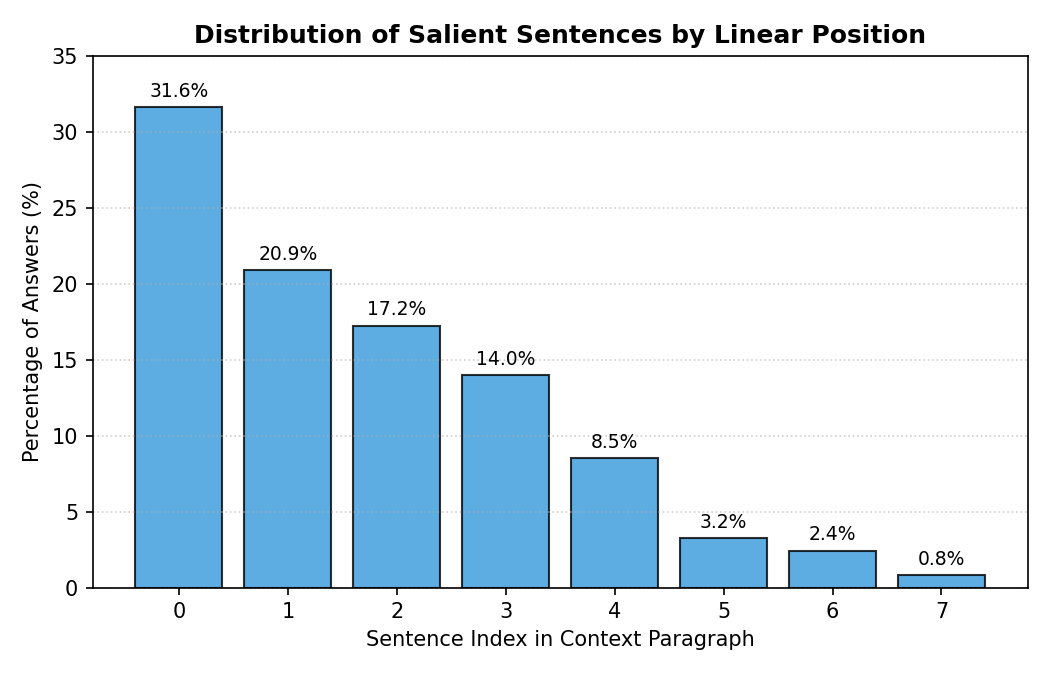
\includegraphics[width=0.65\textwidth]{images/positional_bias.png}
    \caption{Distribution of salient (answer-containing) sentences by their linear index in the SQuAD context paragraph.}
\end{figure}

\textbf{What it shows}: A bar chart of the percentage of answer sentences at each sentence position (index 0--7).\\[4pt]
\textbf{Key pattern}: Index 0 alone accounts for \textbf{31.6\%} of all answers; indices 0--2 together account for \textbf{69.7\%}. The distribution is strongly monotonically decreasing.\\[4pt]
\textbf{Implication}: Any model trained on raw unbalanced data can achieve near-baseline F1 by simply predicting the first two sentences as salient --- a positional shortcut. This is the primary motivation for all five balancing strategies (Pairwise, Cluster, RST-Neighborhood, DSNB).

---

\subsection{Fig 2: Sentence Length Comparison}
\begin{figure}[h!]
    \centering
    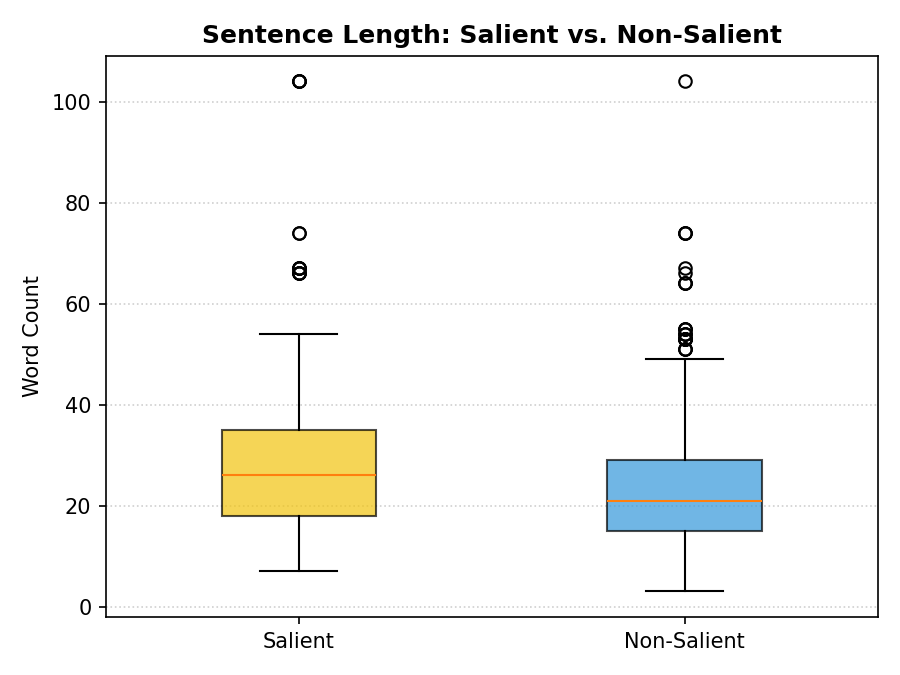
\includegraphics[width=0.55\textwidth]{images/length_comparison.png}
    \caption{Box plot of word count for salient vs.\ non-salient sentences.}
\end{figure}

\textbf{What it shows}: Box plots comparing the distribution of word counts for salient (gold) and non-salient (blue) sentences.\\[4pt]
\textbf{Key pattern}: Salient sentences have a higher median word count ($\approx$28 words) compared to non-salient sentences ($\approx$22 words). Both distributions share similar upper whiskers and outliers.\\[4pt]
\textbf{Implication}: Sentence length is a weak but consistent positive predictor of salience --- answer sentences tend to be more verbose, carrying the specific factual content needed to answer a question. This validates including \texttt{word\_count} and \texttt{char\_count} in the feature set.

---

\subsection{Fig 3: Text Readability (Gunning Fog Index)}
\begin{figure}[h!]
    \centering
    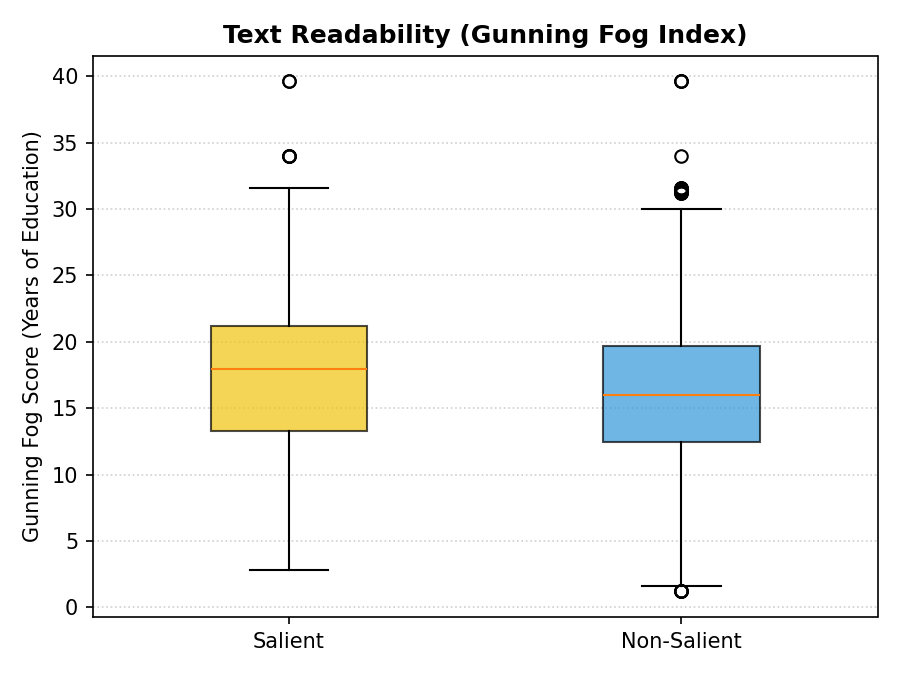
\includegraphics[width=0.55\textwidth]{images/readability_comparison.png}
    \caption{Box plot of the Gunning Fog readability index for salient vs.\ non-salient sentences.}
\end{figure}

\textbf{What it shows}: Box plots of the Gunning Fog Index (a proxy for reading difficulty measured in years of education required) for both classes.\\[4pt]
\textbf{Key pattern}: Salient sentences (median $\approx$18) score slightly higher than non-salient sentences (median $\approx$16). Both classes have high variance and similar extreme outliers at Fog $\approx$40.\\[4pt]
\textbf{Implication}: Answer sentences are marginally more complex --- they use longer words and denser phrasing. The Flesch--Kincaid grade score being the top LR coefficient ($+0.669$) is consistent with this pattern.

---

\subsection{Fig 4: Syntactic Complexity (Dependency Distance)}
\begin{figure}[h!]
    \centering
    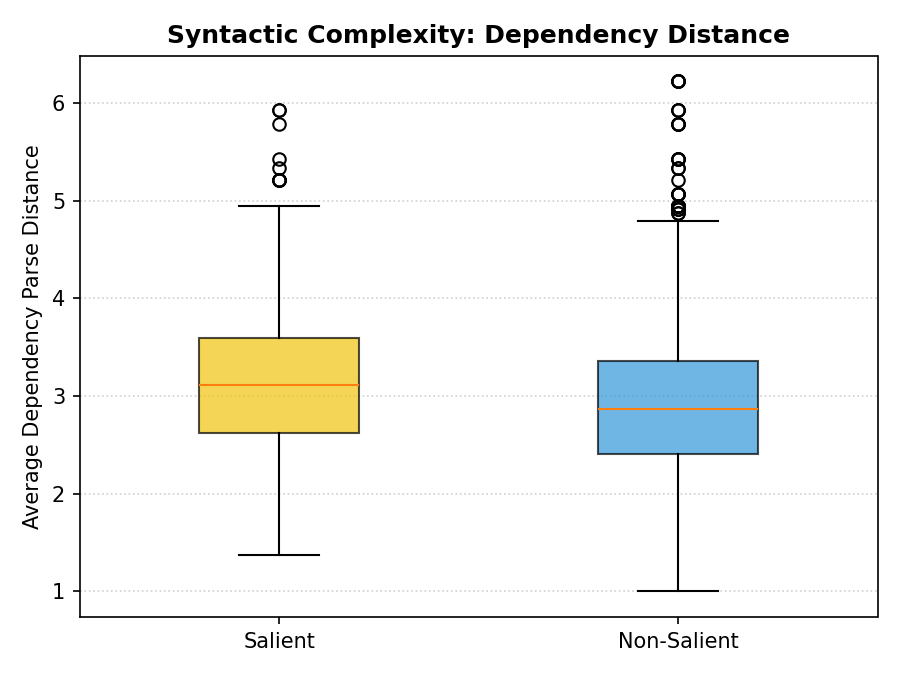
\includegraphics[width=0.55\textwidth]{images/syntactic_complexity.png}
    \caption{Box plot of average dependency parse distance for salient vs.\ non-salient sentences.}
\end{figure}

\textbf{What it shows}: Average dependency distance --- the mean number of words separating a head and its dependent in the dependency parse tree.\\[4pt]
\textbf{Key pattern}: Salient sentences have a marginally higher median dependency distance ($\approx$3.1) than non-salient sentences ($\approx$2.9). Both IQRs heavily overlap.\\[4pt]
\textbf{Implication}: Answer sentences pack more syntactically distant modifier relationships --- a sign of embedded clauses and precise noun phrases (e.g., ``the oxygen transported by haemoglobin''). This feature contributes positively to salience but is not a strong standalone predictor.

---

\subsection{Fig 5: RST Relations Frequency Comparison}
\begin{figure}[h!]
    \centering
    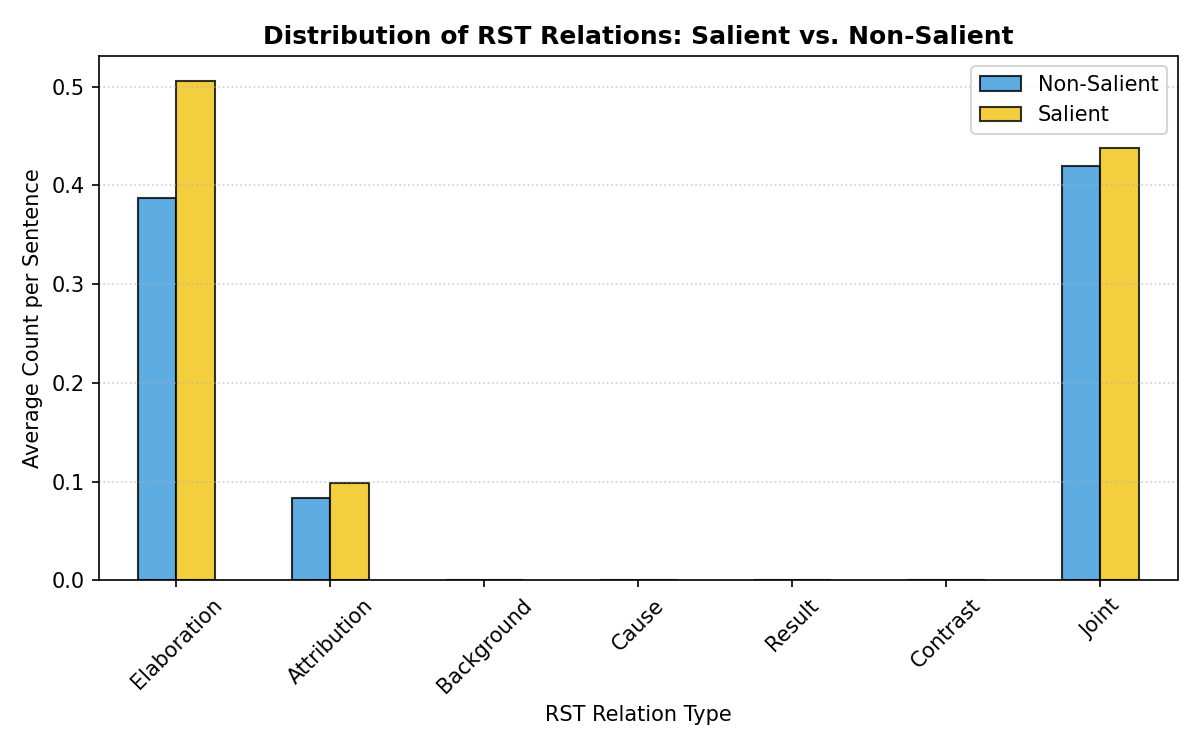
\includegraphics[width=0.7\textwidth]{images/rst_relations_comparison.png}
    \caption{Mean RST relation count per sentence for seven discourse relation types, comparing salient (green) vs.\ non-salient (grey) classes.}
\end{figure}

\textbf{What it shows}: A grouped bar chart of the mean count of seven RST relation types (Elaboration, Attribution, Background, Cause, Result, Contrast, Joint) per sentence for each class.\\[4pt]
\textbf{Key pattern}: Salient sentences have more \textbf{Elaboration} ($0.53$ vs $0.45$) and more \textbf{Joint} ($0.82$ vs $0.72$) relations. Background, Cause, Result, and Contrast relations are nearly zero for both classes.\\[4pt]
\textbf{Implication}: Salient sentences tend to occupy \textit{nucleus} positions in discourse (Elaboration relations attach to a nucleus providing the main fact). Joint relations indicate that answer sentences are frequently structured as paired coordinate clauses --- both facts relevant. Non-salient sentences appear more often as \textit{satellites} providing background context.

---

\subsection{Fig 6: Information Density --- Surprisal Deletion Drop}
\begin{figure}[h!]
    \centering
    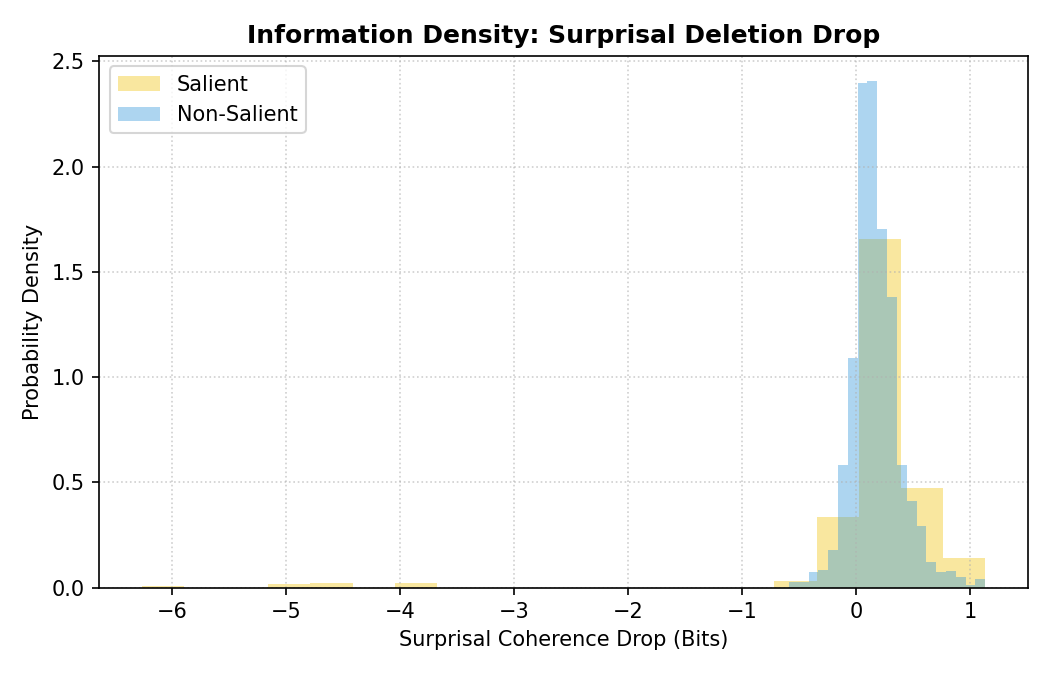
\includegraphics[width=0.7\textwidth]{images/surprisal_distribution.png}
    \caption{Probability density of the GPT-2 coherence drop (in bits) when a sentence is deleted from the context, for salient vs.\ non-salient classes.}
\end{figure}

\textbf{What it shows}: Overlapping histogram of the surprisal coherence drop feature --- the drop in GPT-2 log-probability of the remaining text when a sentence is removed.\\[4pt]
\textbf{Key pattern}: Both classes are tightly concentrated near 0. However, salient sentences (yellow) have a fatter right tail extending beyond $+0.5$ bits, while non-salient sentences (blue) peak more sharply at 0.\\[4pt]
\textbf{Implication}: Deleting a salient sentence causes a measurable disruption in the coherence of surrounding text --- the language model finds the remaining passage harder to predict. This validates the Uniform Information Density (UID) hypothesis: answer sentences are contextual anchors, and removing them breaks the local discourse flow.

---

\subsection{Fig 7: UID Distribution --- Word-Level Surprisal CDFs}
\begin{figure}[h!]
    \centering
    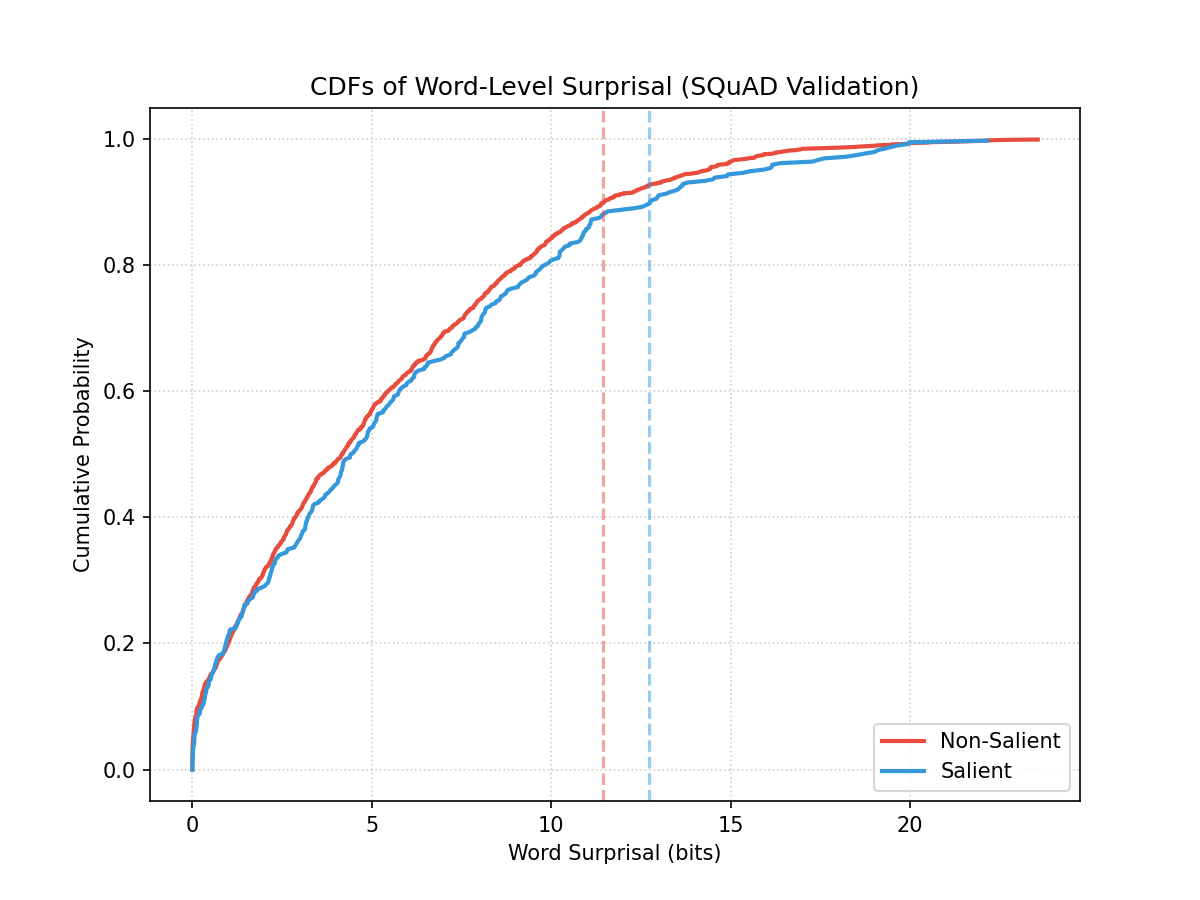
\includegraphics[width=0.7\textwidth]{images/uid_distribution.png}
    \caption{Cumulative Distribution Functions (CDFs) of word-level GPT-2 surprisal for salient (blue) and non-salient (red) sentences, with dashed lines at the median.}
\end{figure}

\textbf{What it shows}: CDFs of word-level surprisal (in bits) across all words in salient vs.\ non-salient sentences. Dashed lines mark the median for each class.\\[4pt]
\textbf{Key pattern}: The salient CDF (blue) lies \textit{to the right} of the non-salient CDF (red) in the tail region (above $\approx$10 bits). The median for salient sentences ($\approx$13 bits) is higher than for non-salient sentences ($\approx$11.5 bits).\\[4pt]
\textbf{Implication}: Salient sentences contain words that are individually more surprising to GPT-2 --- proper nouns, technical terms, and domain-specific facts. This confirms that UID tail percentile features ($P_{90}$, $P_{95}$) are valid signals: answer sentences carry unusually high-surprisal words (the actual facts needed for QA).

---

\subsection{Fig 8: Soft Hybrid Target Label Separability}
\begin{figure}[h!]
    \centering
    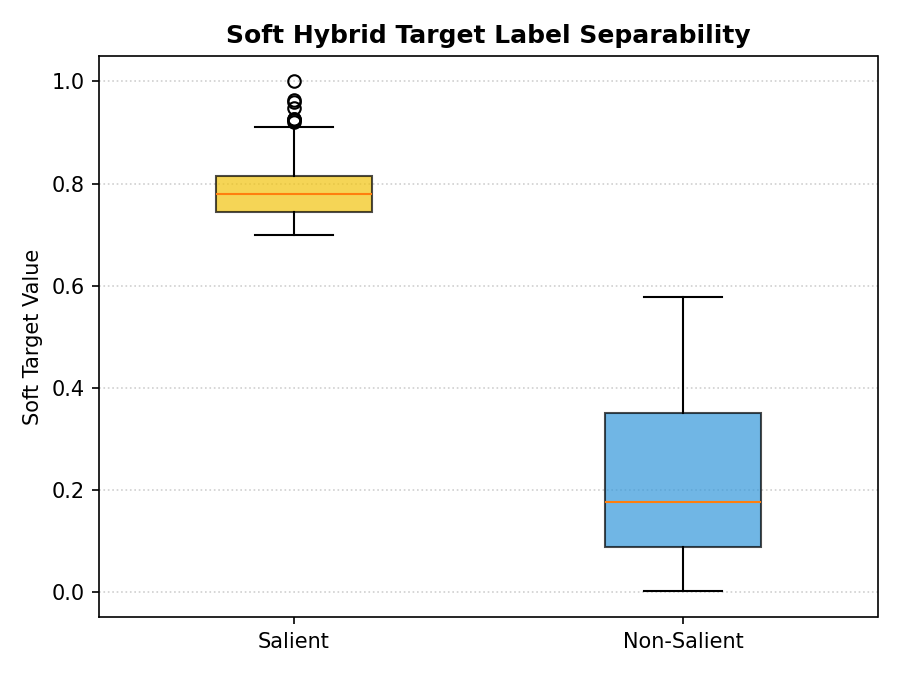
\includegraphics[width=0.55\textwidth]{images/soft_labels_comparison.png}
    \caption{Box plot of the soft hybrid target label values for salient vs.\ non-salient sentences.}
\end{figure}

\textbf{What it shows}: A box plot comparing the distribution of the soft target label values (ranging 0--1) between the two classes.\\[4pt]
\textbf{Key pattern}: Salient sentences have a tightly concentrated soft label around $0.78$--$0.80$ (IQR: $0.73$--$0.83$). Non-salient sentences spread widely from $0.10$ to $0.35$ (IQR: $0.10$--$0.35$), with median $\approx 0.19$.\\[4pt]
\textbf{Implication}: The soft label construction (combining hard binary label with continuous RST and surprisal evidence) creates excellent class separability. The gap between median soft labels ($0.79$ vs $0.19$) confirms that the hybrid labelling scheme successfully encodes discourse and information-density evidence into a continuous signal that is well-separated by class.

---

\subsection{Fig 9: Pearson Correlation of Features with Salience}
\begin{figure}[h!]
    \centering
    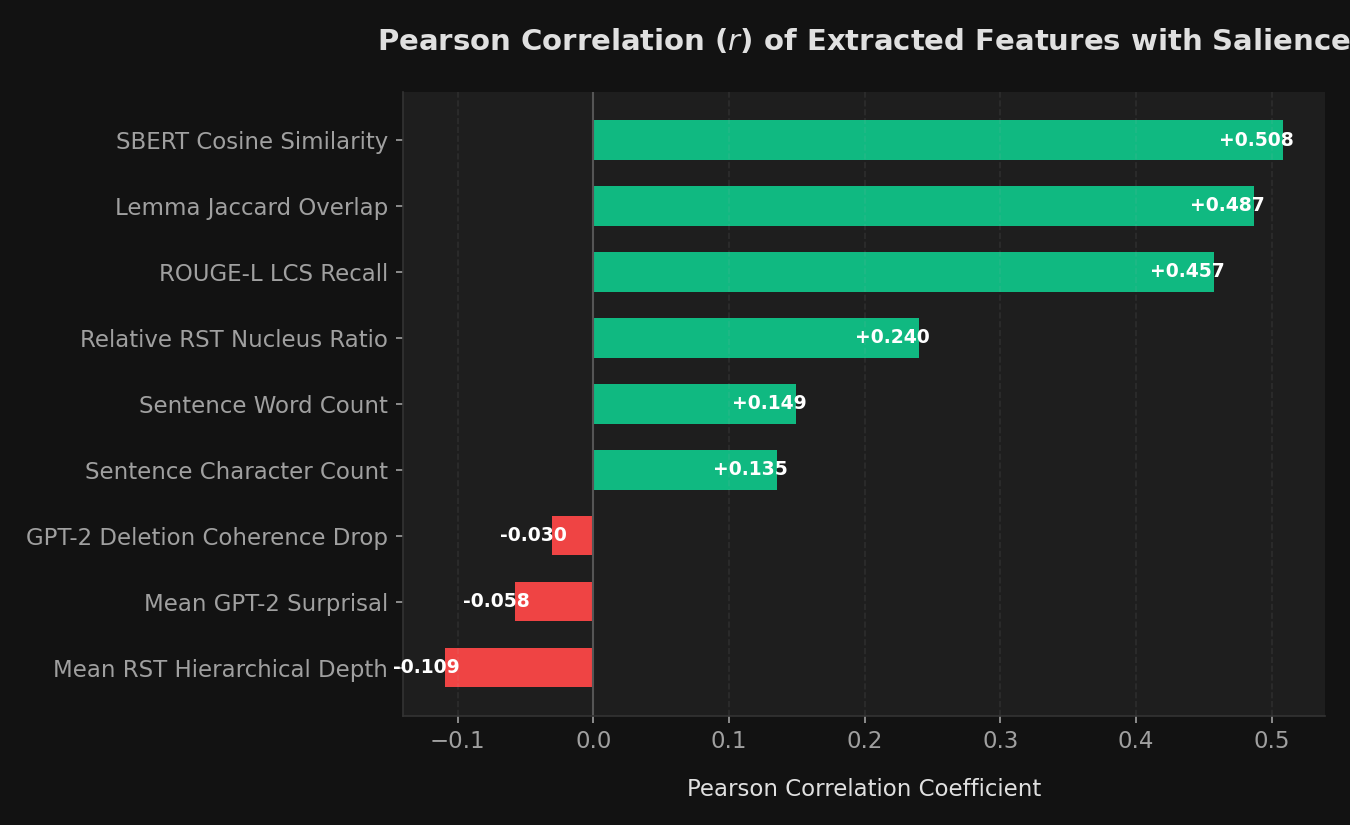
\includegraphics[width=0.7\textwidth]{images/feature_correlations.png}
    \caption{Horizontal bar chart of Pearson $r$ between each extracted feature and the binary salience label.}
\end{figure}

\textbf{What it shows}: The Pearson correlation coefficient between individual features and the salience target. Green bars indicate positive correlation; red bars indicate negative correlation.\\[4pt]
\textbf{Key pattern}: The three strongest correlations --- SBERT Cosine Similarity ($+0.508$), Lemma Jaccard Overlap ($+0.487$), ROUGE-L LCS Recall ($+0.457$) --- are all \textbf{alignment features} that measure sentence-to-question similarity. The strongest \textit{non-alignment} feature is RST Nucleus Ratio ($+0.240$). Mean RST Hierarchical Depth is the strongest negative predictor ($-0.109$).\\[4pt]
\textbf{Implication}: This plot is the core motivation for the difficulty of the problem. The most predictive features are excluded by the query-independent constraint. Our models must operate with features whose individual correlation with salience is at most $+0.24$. The moderate F1 scores (0.30--0.35) across all models are therefore expected and justify the complexity of the neural fusion architectures.

---

\subsection{Fig 10: Pearson Correlation Matrix of Key Features}
\begin{figure}[h!]
    \centering
    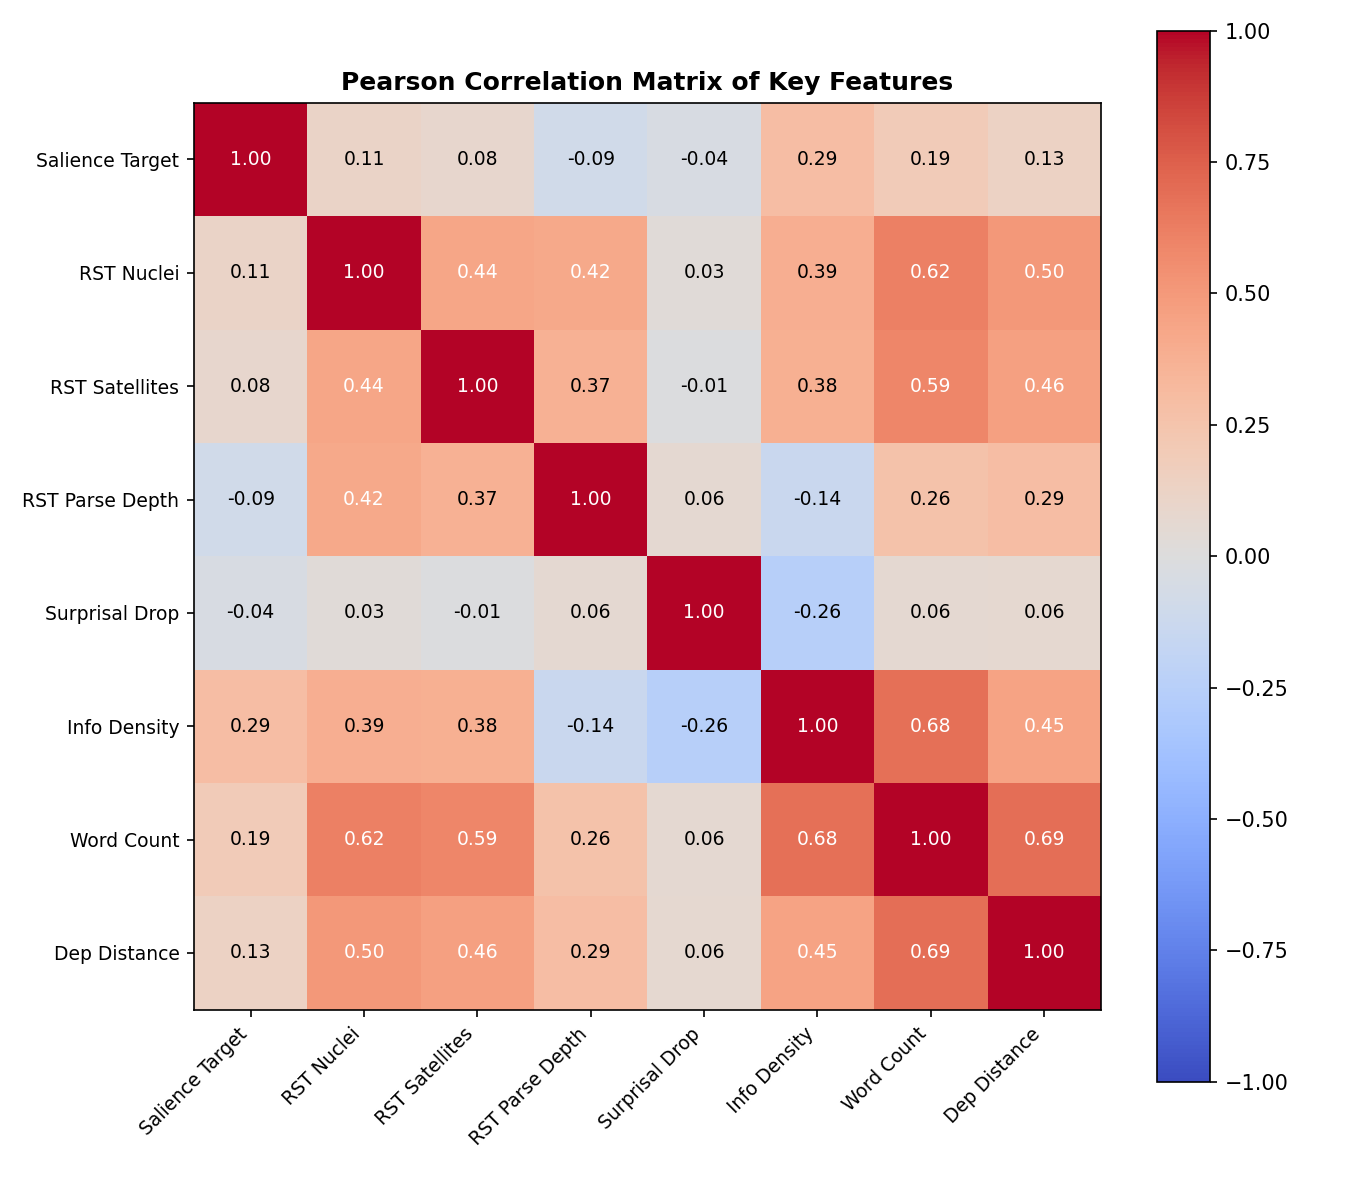
\includegraphics[width=0.75\textwidth]{images/correlation_heatmap.png}
    \caption{Pearson correlation matrix between the salience target and seven key features.}
\end{figure}

\textbf{What it shows}: A symmetric heatmap of Pearson $r$ values between all pairs of: Salience Target, RST Nuclei, RST Satellites, RST Parse Depth, Surprisal Drop, Info Density (surprisal ratio), Word Count, and Dependency Distance.\\[4pt]
\textbf{Key patterns}:
\begin{itemize}
    \item \textbf{Info Density $\leftrightarrow$ Salience}: $r = +0.29$ --- strongest non-alignment predictor of salience.
    \item \textbf{Word Count $\leftrightarrow$ Info Density}: $r = +0.68$ --- high co-linearity, as longer sentences accumulate more surprisal.
    \item \textbf{RST Parse Depth $\leftrightarrow$ Salience}: $r = -0.09$ --- deeper tree position weakly reduces salience (deeper = more satellite).
    \item \textbf{RST Nuclei $\leftrightarrow$ Word Count}: $r = +0.62$ --- longer sentences have more discourse relations.
    \item \textbf{Surprisal Drop $\leftrightarrow$ Info Density}: $r = -0.26$ --- sentences with high relative surprisal tend to show smaller coherence drops (they are already surprising in context).
\end{itemize}
\textbf{Implication}: The moderate inter-feature correlations confirm that each feature family contributes partially independent signal. This justifies the Combined LR model (Config 5) which benefits from all five feature families without severe multi-collinearity.

---

\subsection{Fig 11: LGSM Gating Analysis}
\begin{figure}[h!]
    \centering
    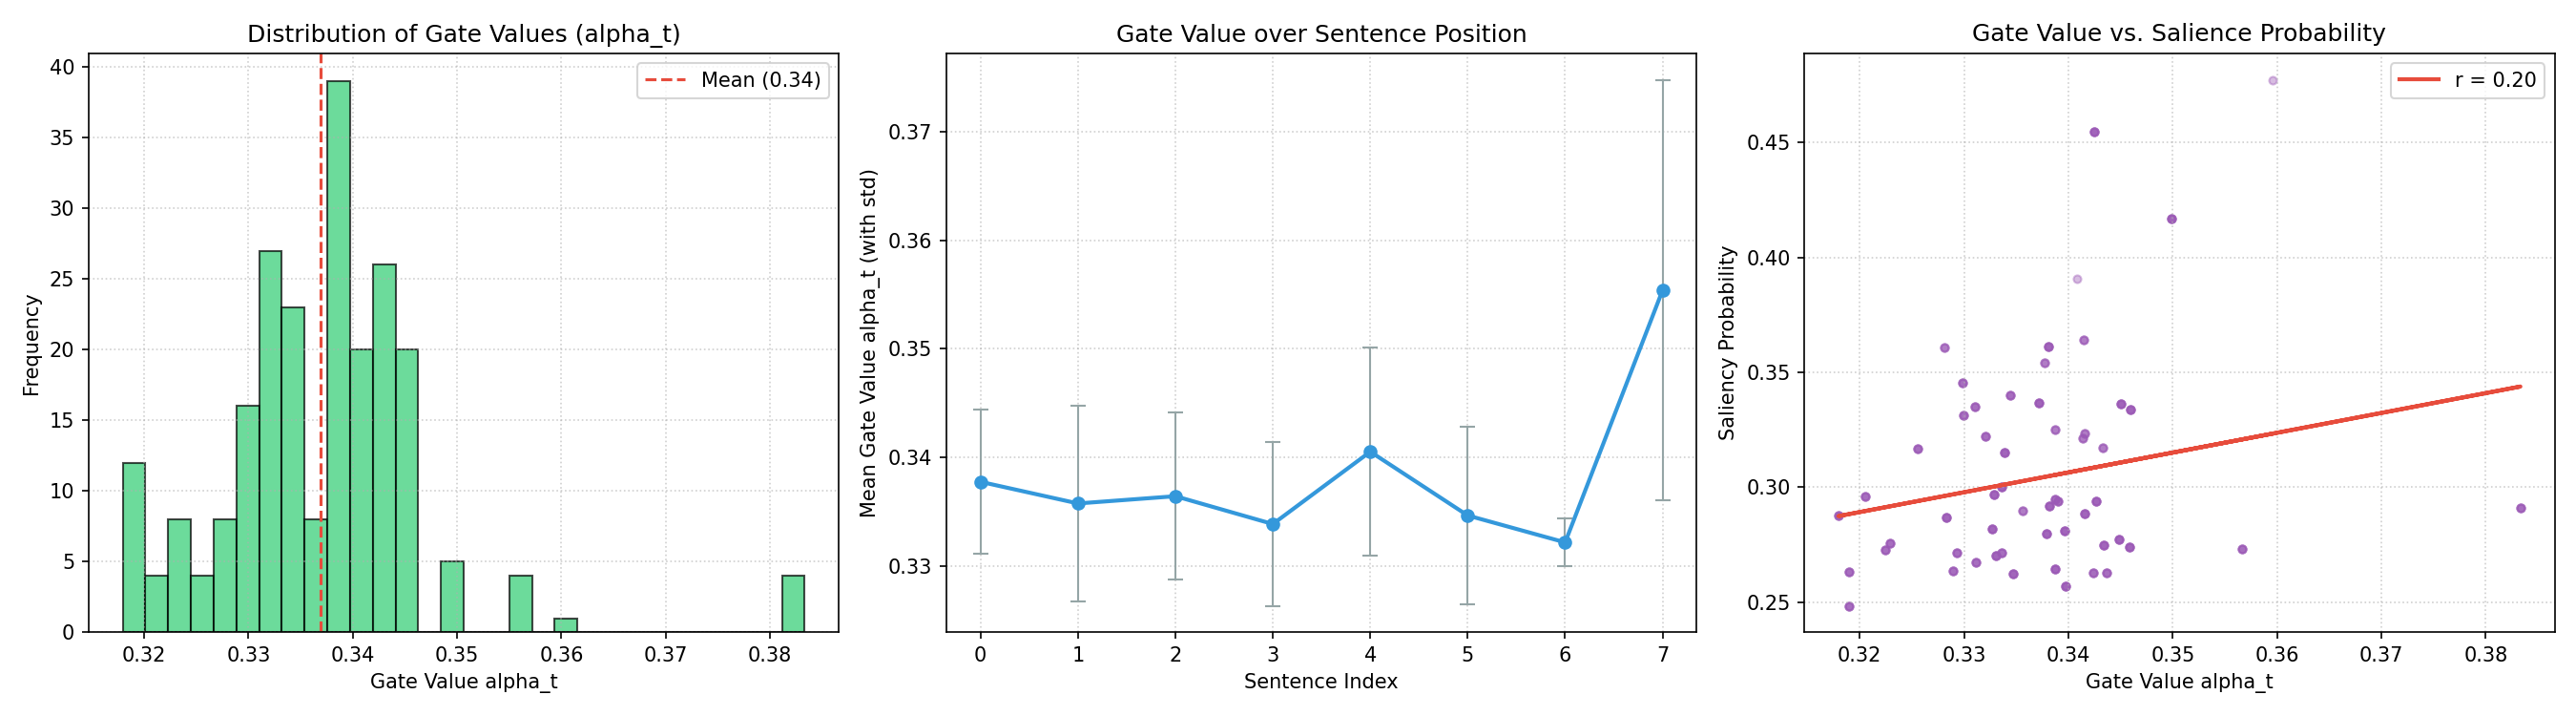
\includegraphics[width=\textwidth]{images/gating_progression.png}
    \caption{Three-panel analysis of the LGSM scalar gate $\alpha_t$: (left) histogram of gate values, (centre) mean gate value by sentence position with error bars, (right) scatter of gate value vs.\ predicted salience probability.}
\end{figure}

\textbf{What it shows}: Three diagnostic panels for the LGSM model's learned scalar gate $\alpha_t \in (0,1)$ which controls reliance on explicit features vs.\ BERT CLS embeddings.\\[4pt]
\textbf{Panel 1 --- Distribution}: Gate values are tightly concentrated around the mean $0.34$ (dashed red line), with most values between $0.32$--$0.36$. Very few sentences push above $0.37$.\\[4pt]
\textbf{Panel 2 --- Gate over Position}: Mean gate value is nearly constant across sentence indices 0--6 ($\approx 0.335$), but jumps sharply at index 7 ($\approx 0.354$). Error bars show high within-position variance.\\[4pt]
\textbf{Panel 3 --- Gate vs.\ Salience}: A positive correlation ($r = 0.20$, $p < 0.002$) between gate value and predicted salience probability --- higher reliance on explicit features correlates with higher predicted salience.\\[4pt]
\textbf{Implication}: The LGSM gate has learned that explicit features are slightly more diagnostic for later-position sentences. More importantly, sentences that the model predicts as salient are associated with higher gate values, confirming that the explicit feature stream (RST + surprisal) carries positive salience signal even in the sequence-level model.

---

\subsection{Fig 12: Threshold Sensitivity Analysis}
\begin{figure}[h!]
    \centering
    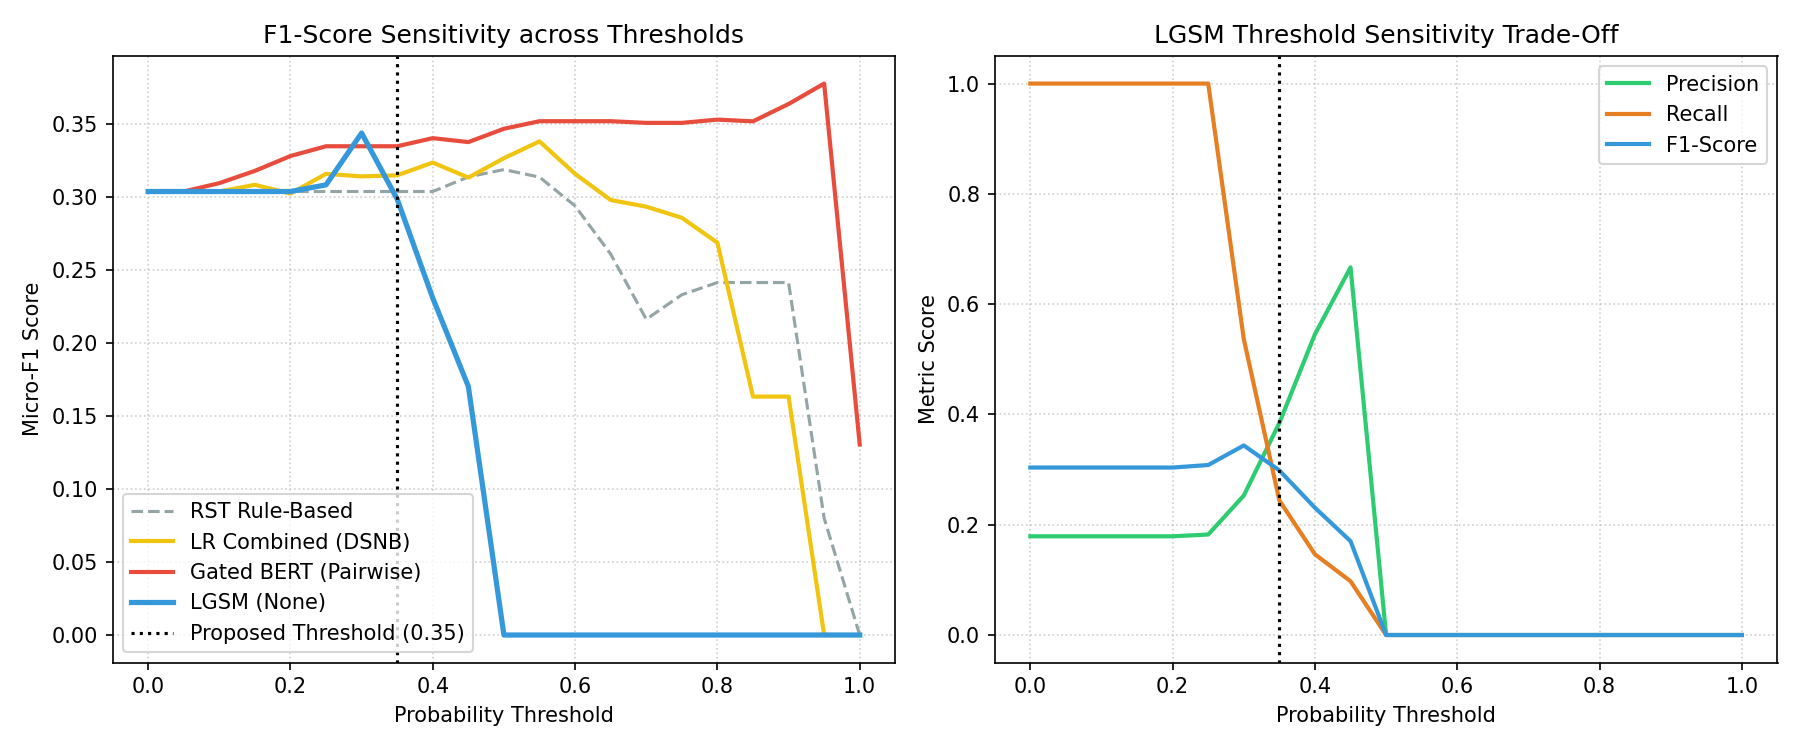
\includegraphics[width=\textwidth]{images/threshold_sensitivity.png}
    \caption{(Left) Micro-F1 vs.\ probability threshold for all four key models. (Right) Precision, Recall, and F1 vs.\ threshold for LGSM only.}
\end{figure}

\textbf{What it shows}: How each model's F1 score changes as the decision threshold (probability cutoff for predicting salience) is swept from 0.0 to 1.0.\\[4pt]
\textbf{Key patterns}:
\begin{itemize}
    \item \textbf{Gated BERT (red)}: Continuously rises from $F_1 = 0.30$ at threshold $0.0$ to $F_1 = 0.377$ at threshold $\approx 0.95$ before collapsing at 1.0. This indicates well-calibrated probability scores --- raising the threshold keeps filtering true negatives.
    \item \textbf{LR Combined (yellow)}: Peaks at threshold $\approx 0.55$--$0.60$ ($F_1 \approx 0.338$) then gradually decreases.
    \item \textbf{RST Rule-Based (dashed grey)}: Completely flat at $F_1 \approx 0.30$ from 0.0 to 0.7, then collapses --- confirming it is a hard rule, not a probability model.
    \item \textbf{LGSM (blue)}: Peaks sharply at threshold $= 0.30$ ($F_1 = 0.344$), collapses to zero by $0.50$ --- most predictions are clustered in a narrow range $0.25$--$0.40$.
\end{itemize}
\textbf{Right panel}: LGSM's precision rises steeply from $0.18$ at $\tau=0$ to $0.67$ at $\tau=0.45$, while recall drops from $1.0$ to near $0$. Peak F1 $= 0.344$ occurs at $\tau = 0.30$.\\[4pt]
\textbf{Implication}: The chosen threshold $\tau = 0.35$ is a cross-model compromise. For LGSM specifically, $\tau = 0.30$ is optimal. The near-flat shape of Gated BERT implies its scores are discriminative across the full range, making it robust to threshold choice.

---

\subsection{Fig 13: Top-K Recall Curve}
\begin{figure}[h!]
    \centering
    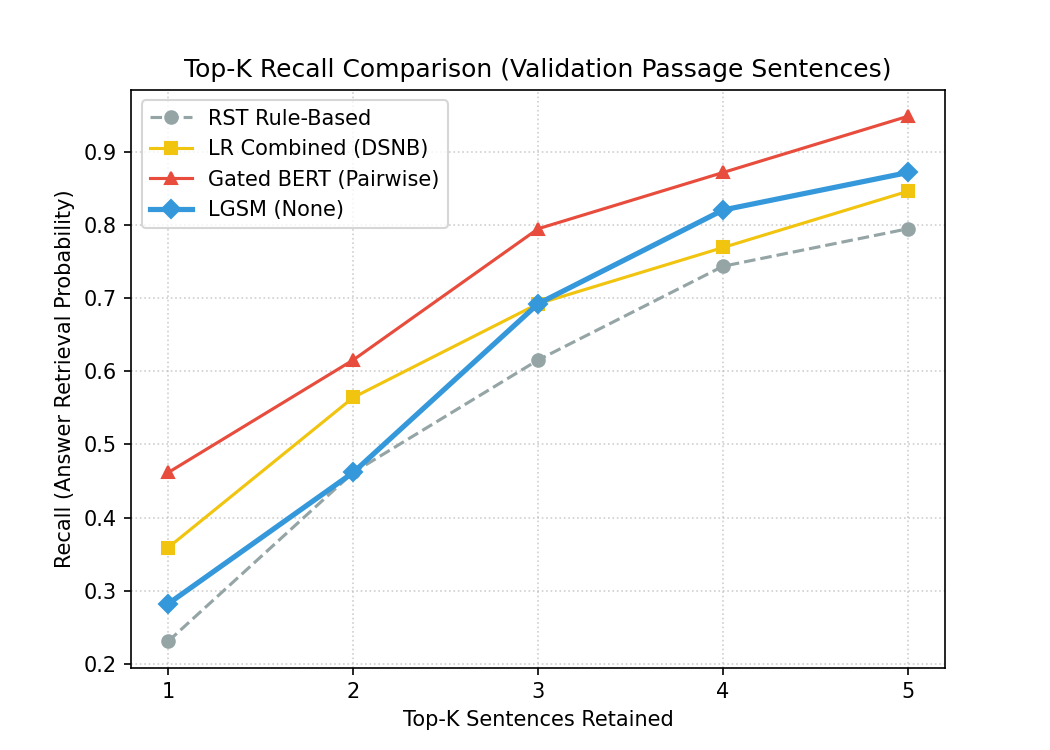
\includegraphics[width=0.7\textwidth]{images/top_k_recall_curve.png}
    \caption{Top-K recall comparison: probability of retrieving the true answer sentence within the top-$K$ ranked predictions, for $K = 1$ to $5$.}
\end{figure}

\textbf{What it shows}: For each model, the probability that at least one true salient sentence is included when only the top-$K$ highest-scored sentences are retained.\\[4pt]
\textbf{Key patterns}:
\begin{itemize}
    \item \textbf{Gated BERT (red)}: Dominates at every $K$. Top-1 recall = $0.46$, reaching $0.95$ at $K=5$.
    \item \textbf{LR Combined (yellow)}: Top-1 = $0.36$, reaches $0.85$ at $K=5$.
    \item \textbf{LGSM (blue)}: Slightly behind LR at low $K$ (Top-1 = $0.29$), nearly catches up by $K=5$ ($0.87$).
    \item \textbf{RST Rule-Based (dashed grey)}: Worst at every $K$ (Top-1 = $0.23$, $K=5$ = $0.80$) due to poor score discrimination.
\end{itemize}
\textbf{Implication}: For a downstream QG pipeline, the practically important figure is Top-2 or Top-3 recall (how many candidate sentences to send to the question generator). Gated BERT achieves $0.62$ recall at $K=2$ and $0.80$ at $K=3$, meaning 80\% of QG contexts would already contain the answer sentence with only 3 candidates. This strongly motivates Gated BERT as the preferred selector for the downstream pipeline.

\end{document}
